\documentclass[12pt]{article}
\usepackage[brazilian]{babel}
\usepackage[utf8]{inputenc}
\usepackage[T1]{fontenc}
\usepackage{amsmath}
\usepackage{float}
\usepackage{graphicx}
\usepackage{hyperref}

\sloppy

\title{Mr. Monkey - The Vampire Bunny Hunter \\ Entretenimento Digital}

\author{Matthias Oliveira de Nunes}

\begin{document}

\maketitle

\begin{abstract}

Um jogo em que se pode explorar um mapa lutando contra vários monstros
poderosos. É um plataforma de ação com exploração.

\end{abstract}

\section{Tipo de jogo}

Um plataforma de ação em 2D.

\section{Descrição Geral}

Esse jogo foi inspirado na série $Castlevania$, tendo como personagem
controlável um macaco caçador de coelhos vampiros. O objetivo principal do jogo
é eliminar todos os inimigos, sendo essa a condição para passar para a próxima
fase.

\section{Gameplay}

Os comandos do jogo serão feitos através do teclado. As teclas $\uparrow
\leftarrow \downarrow \rightarrow$ representam, respectivamente: pulo; andar
para a esquerda; erguer as mãos; andar para a direita.

\section{Mapa do Ambiente}

\subsection{Fase 1}

\begin{figure}[H]
        \centering
        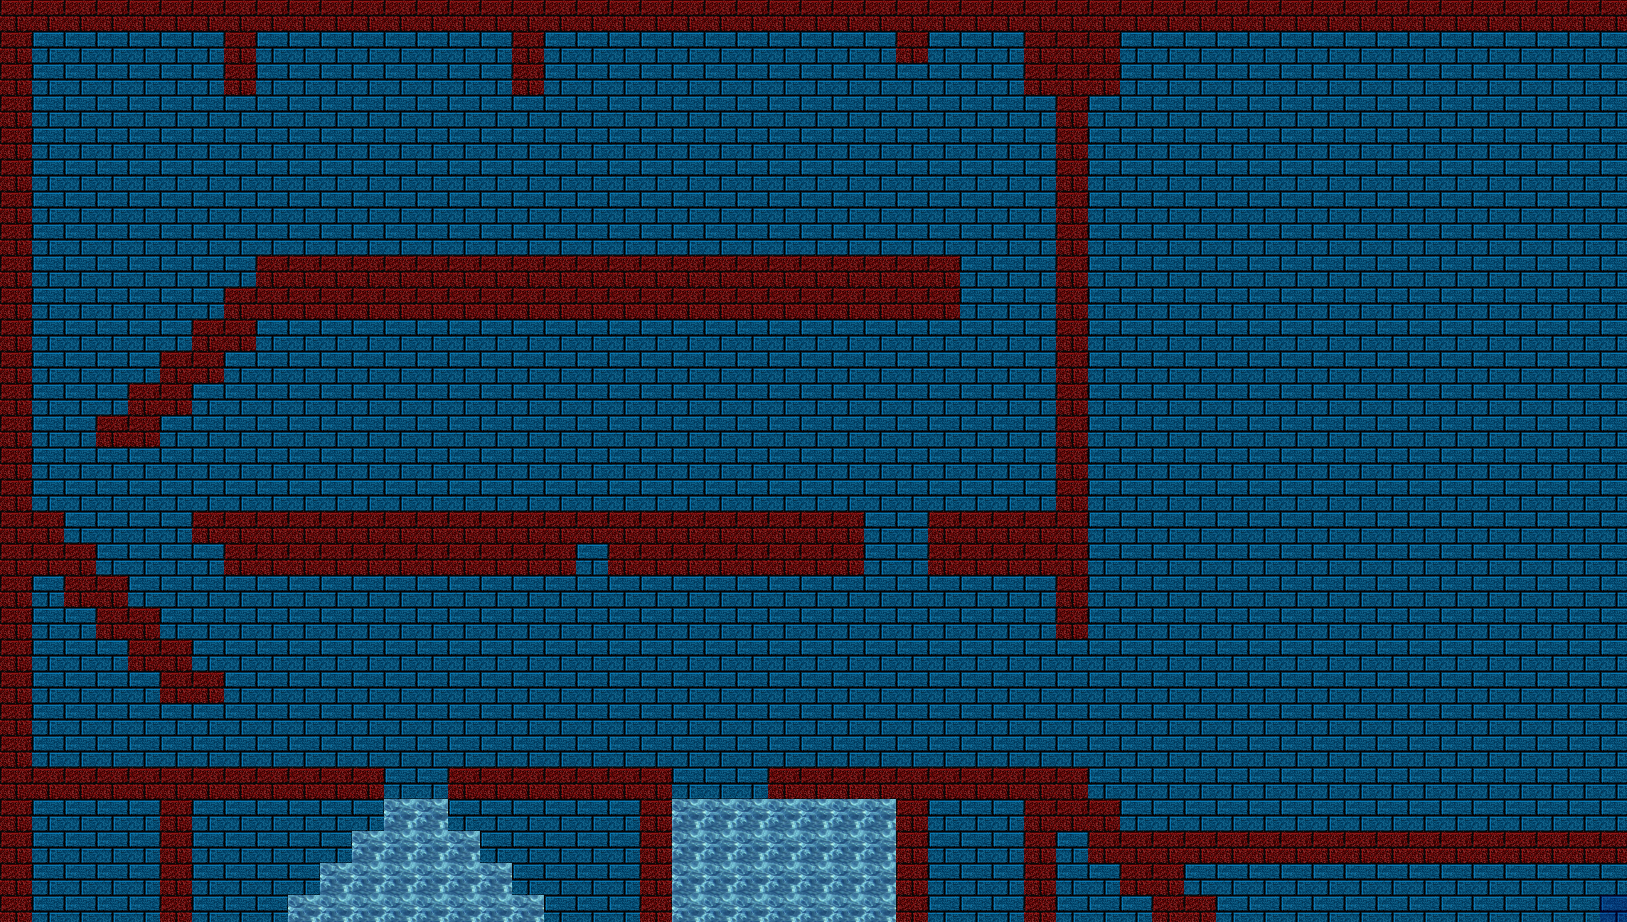
\includegraphics[width=100mm]{map1.png}
        \caption{Fase 1}
        \label{m1}
\end{figure}

Após matar todos os inimigos na fase 1, o jogador é levado à fase dois.

\subsection{Fase 2}

\begin{figure}[H]
        \centering
        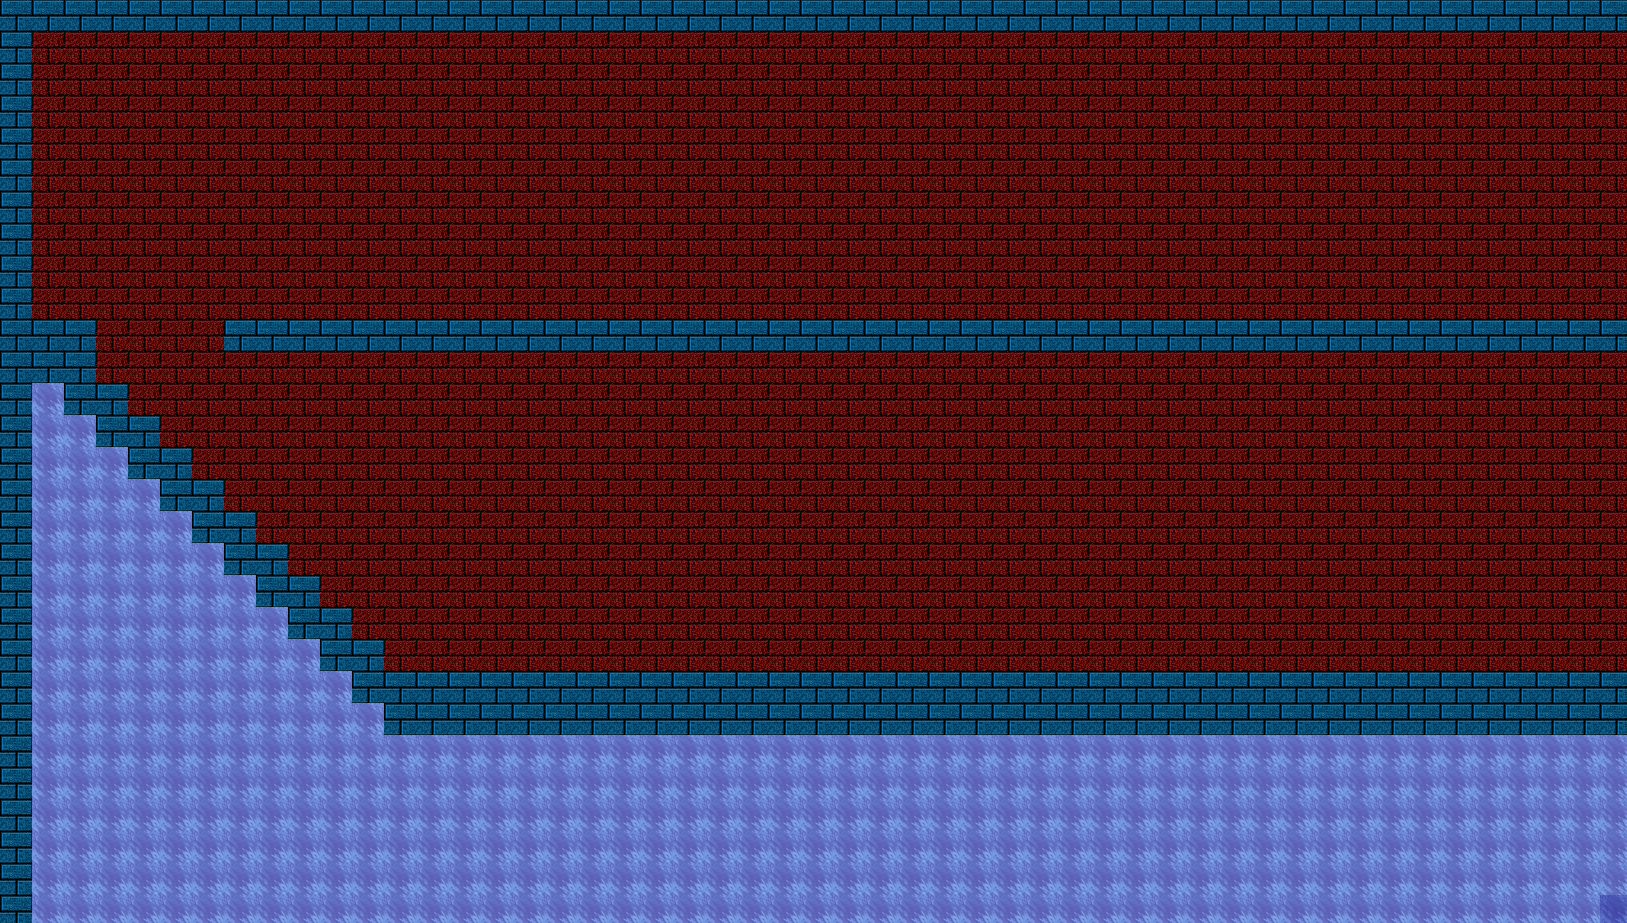
\includegraphics[width=100mm]{map2.png}
        \caption{Fase 2}
        \label{m2}
\end{figure}

Após matar todos os inimigos na fase 2, o jogador virou o jogo.

\section{Requisitos de Audio}

\subsection{Músicas}

Como trilha sonora foram usadas duas músicas, sendo elas:

\begin{enumerate}
  \item Durarara!! OST [Vol.1] - Ikebukuru West Exit Five-way Intersection
  \item Durarara!! OST [Vol.1] - On Tuesday Night
\end{enumerate}

\subsection{Sonoplastia}

Foram utilizados um som de macaco e outro de cavalo, eles foram retirados
\href{http://www.wavsource.com/animals/animals.htm}{desse site.}

\emph{http://www.wavsource.com/animals/animals.htm}

\section{Lista de Assets}

Softwares utilizados:

\begin{itemize}
  \item \href{http://www.codeblocks.org/}{Code::Blocks}
  \item \href{http://www.sfml-dev.org/}{SFML}
  \item \href{https://www.codeandweb.com/texturepacker}{TexturePacker}
  \item \href{http://www.mapeditor.org/}{Tiled}
\end{itemize}

\subsection{Sprites}
\label{sub:Sprites}

As sprites utilizadas vieram do
\href{http://www.gameartguppy.com/}{GameArtGuppy}.

\begin{figure}[H]
        \centering
        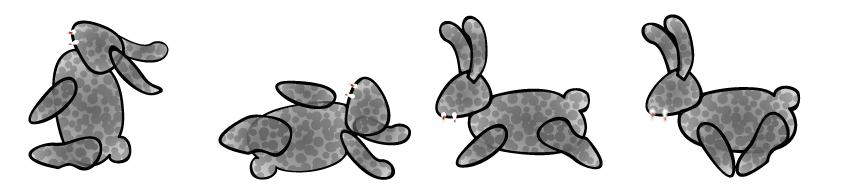
\includegraphics[width=100mm]{bunny.png}
        \caption{Vampire Bunny}
        \label{bu}
\end{figure}

\begin{figure}[H]
        \centering
        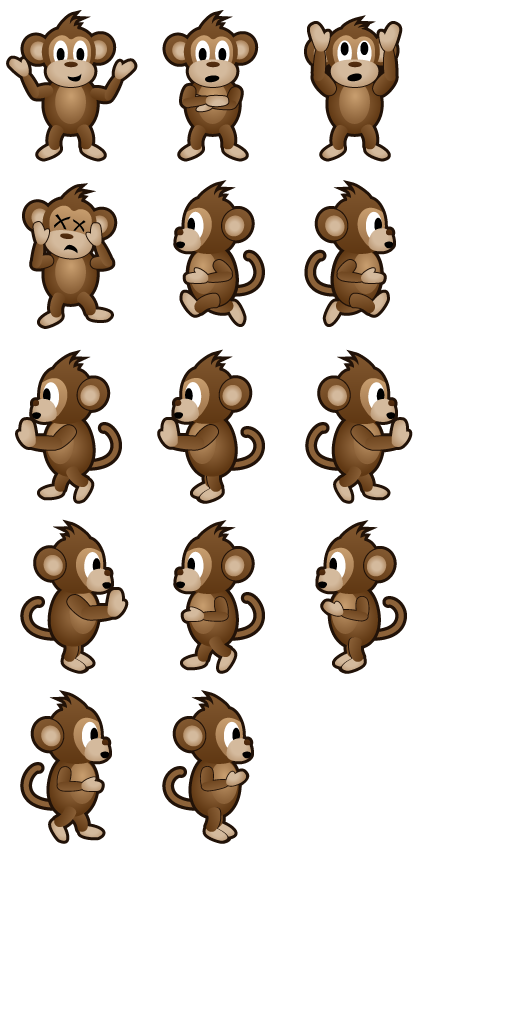
\includegraphics[width=100mm]{monkey.png}
        \caption{Monkey}
        \label{mo}
\end{figure}

\end{document}
